\documentclass[a4paper,11pt]{article}

% ==========================================
% 1. CONFIGURACIÓN DEL PROYECTO
% ==========================================
\newcommand{\titol}{Motor de Recomendación Cinematográfica de Altas Prestaciones Basado en Redes Neuronales y Metadatos Heterogéneos}
\newcommand{\subtitol}{Propuesta de Proyecto: Caracterización de Datos Masivos, Revisión del Estado del Arte y Justificación Tecnológica}
\newcommand{\assignatura}{Computació d'Altes Prestacions i Intel·ligència Artificial (CPIA)}
\newcommand{\assignaturaCurt}{CPIA (UPC)}
\newcommand{\universitat}{Universitat Politècnica de Catalunya}
\newcommand{\escola}{ETSETB / FIB}
\newcommand{\autorA}{Arnau Montull}
\newcommand{\autorB}{Uriel Martínez}

% ==========================================
% 2. PAQUETES Y CONFIGURACIÓN TIPOGRÁFICA
% ==========================================
\usepackage[utf8]{inputenc}
\usepackage[T1]{fontenc}
\usepackage{lmodern}
\usepackage[spanish,es-nodecimaldot]{babel}

% Estandarizar nombre de tablas
\addto\captionsspanish{\renewcommand{\tablename}{Tabla}}

\usepackage{amsmath, amssymb, amsfonts, amsthm}
\usepackage{mathtools}
\usepackage{geometry}
\geometry{
    left=2.1cm,
    right=2.1cm,
    top=2.2cm,
    bottom=2.2cm,
    headheight=14.5pt
}

\usepackage{microtype}
\usepackage{graphicx}
\usepackage{parskip}   
\usepackage{caption}
\usepackage{subcaption} 
\usepackage{fancyhdr}   
\usepackage{xcolor}
\usepackage{booktabs}
\usepackage{tabularx}  
\usepackage{array}
\usepackage{siunitx}
\sisetup{output-decimal-marker = {.}}

% Control fino de distancias para figuras flotantes
\setlength{\textfloatsep}{10pt plus 2pt minus 2pt}
\setlength{\intextsep}{9pt plus 2pt minus 2pt}
\setlength{\floatsep}{8pt plus 2pt minus 2pt}

% Hipervínculos
\usepackage{hyperref}
\hypersetup{
    colorlinks=true,
    linkcolor=blue!70!black,
    citecolor=green!50!black,
    urlcolor=blue!80!black
}

% Cabeceras y pies de página
\pagestyle{fancy}
\fancyhf{}
\lhead{\small \textbf{\assignaturaCurt}}
\rhead{\small \autorA, \autorB}
\cfoot{\small \thepage}
\renewcommand{\headrulewidth}{0.4pt}

% Configuración para código fuente
\usepackage{listings}
\definecolor{mGreen}{rgb}{0,0.55,0}
\definecolor{mGray}{rgb}{0.45,0.45,0.45}
\definecolor{mPurple}{rgb}{0.55,0,0.75}
\definecolor{codeBackground}{rgb}{0.97,0.98,0.99}

\lstset{
    language=C++,
    backgroundcolor=\color{codeBackground},   
    commentstyle=\color{mGreen}\itshape,
    keywordstyle=\color{blue}\bfseries,
    numberstyle=\tiny\color{mGray},
    stringstyle=\color{mPurple},
    basicstyle=\ttfamily\footnotesize, 
    breakatwhitespace=false,         
    breaklines=true,                 
    captionpos=b,                    
    keepspaces=true,                 
    numbers=left,                    
    numbersep=8pt,                  
    tabsize=2,
    frame=single,                    
    rulecolor=\color{black!15},
    xleftmargin=16pt,
    framexleftmargin=6pt
}

% ==========================================
% 3. INICIO DEL DOCUMENTO
% ==========================================
\begin{document}

% --- PORTADA ---
\begin{titlepage}
    \thispagestyle{empty}
    \centering
    \vspace*{0.2cm}
    
\includegraphics[width=0.16\textwidth]{Logo_UPC.svg.png}\\[0.3cm]
    
    {\large \textbf{\universitat}}\\[0.12cm]
    {\normalsize \escola}\\[0.9cm]
    
    \rule{\textwidth}{0.6pt}\\[0.35cm]
    {\LARGE \textbf{\titol}}\\[0.25cm]
    {\large \subtitol}\\[0.15cm]
    \rule{\textwidth}{0.6pt}\\[0.7cm]
    
    {\large \textbf{\assignatura}}\\[0.45cm]
    {\large \textbf{Autores:}}\\[0.12cm]
    {\large \autorA}\\[0.08cm]
    {\large \autorB}\\[1.2cm]
    
    \vfill
    
\includegraphics[width=0.12\textwidth]{logo-enginyeria-fisica.jpg}\\[0.25cm]
    {\normalsize \today}
\end{titlepage}

\clearpage

% ==========================================
% SECCIÓN 1: DEFINICIÓN DEL PROBLEMA
% ==========================================
\section{Definición del Problema a Resolver}

\subsection{La Perspectiva del Usuario: La Fatiga de Elección}
En la actualidad, uno de los mayores inconvenientes al abrir una plataforma de contenidos audiovisuales es la llamada fatiga de decisión: los usuarios a menudo invierten más tiempo navegando por menús y carruseles interminables que disfrutando de una película. La mayoría de las recomendaciones que aparecen en pantalla suelen percibirse como poco atractivas, irrelevantes o repetitivas, mostrando una y otra vez los mismos éxitos comerciales. 

El usuario busca descubrir obras que encajen verdaderamente con su gusto personal, incluyendo cine de autor o títulos periféricos de calidad, pero el volumen inmanejable de los catálogos modernos convierte la búsqueda manual en una experiencia lenta y poco satisfactoria.

\subsection{Dificultades Técnicas al Diseñar la Solución}
Hacer una recomendación acertada y personalizada no es trivial debido a las limitaciones estructurales que presentan los datos a gran escala:

\begin{enumerate}
    \item \textbf{Casi nadie ha visto casi nada (Esparcidad masiva):} En un catálogo con más de $80\,000$ títulos, una persona promedio evalúa solo unas pocas decenas o cientos de obras. Esto significa que más del $99.8\%$ de la matriz de interacciones carece de datos. Los algoritmos clásicos de filtrado colaborativo tienen dificultades para inferir relaciones cuando coinciden tan pocas valoraciones entre usuarios.
    
    \item \textbf{Siempre se recomienda lo mismo (Sesgo de popularidad):} El análisis de los datos revela que el $10\%$ de las películas comerciales concentra más del $95\%$ de todas las calificaciones. Como consecuencia directa, los modelos estándar tienden a recomendar de forma redundante títulos muy votados (\textit{blockbusters}) para maximizar su probabilidad de acierto global, invisibilizando miles de películas valiosas de la cola larga (\textit{long-tail}).
    
    \item \textbf{El reto de los usuarios reales y el arranque en frío (\textit{Cold-Start}):} Cuando se añade una película recién estrenada o se incorpora un usuario nuevo, el sistema carece de historial acumulado. Un caso representativo en la comunidad de ciencia de datos es el proyecto de Sam Learner en Kaggle (\textit{Letterboxd Movie Ratings Data}), donde se recopilaron las valoraciones de los $4\,000$ usuarios más activos de Letterboxd. Cuando usuarios reales intentan conectar su perfil para recibir recomendaciones basadas en su diario personal (\textit{diary}), los modelos basados únicamente en IDs de usuario colapsan si no son capaces de procesar secuencias arbitrarias y asociarlas con los metadatos y sinopsis del catálogo.
    
    \item \textbf{Tiempos de respuesta lentos (Latencia y cómputo en CPU):} Comparar el perfil de un usuario contra decenas de miles de películas evaluando redes neuronales completas en tiempo real genera cuellos de botella inasumibles para un servicio interactivo. La solución exige desacoplar el cálculo pesado, precomputar los vectores de las películas y emplear paralelismo multihilo y vectorización en CPU para responder en pocos milisegundos.
\end{enumerate}

\subsection{Objetivo del Sistema}
En lugar de plantear una regresión para predecir la nota exacta de cada película, el sistema se enfoca como un problema de \textbf{Aprendizaje de Ordenamiento (\textit{Learning to Rank}) y Recuperación Top-$K$}. 

Formalmente, el sistema proyecta tanto al usuario $u$ como a cada película $i$ a un espacio métrico latente compartido $\mathbb{R}^d$ ($d \ll M$). A partir de estas representaciones se calcula una puntuación de afinidad $\hat{s}(u, i)$ para ordenar el catálogo, asegurando que las obras relevantes para el usuario ($\mathcal{I}_u^+$) se sitúen por delante del resto del inventario no observado o irrelevante:
\begin{equation}
    \hat{s}(u, i) > \hat{s}(u, j) \quad \forall \, i \in \mathcal{I}_u^+, \; j \in \mathcal{I} \setminus \mathcal{I}_u^+
    \label{eq:ranking_obj}
\end{equation}

El propósito final es devolver una selección reducida, diversa y personalizada de películas en tiempo real, ahorrando tiempo de búsqueda al espectador.

\begin{figure}[!htbp]
    \centering
    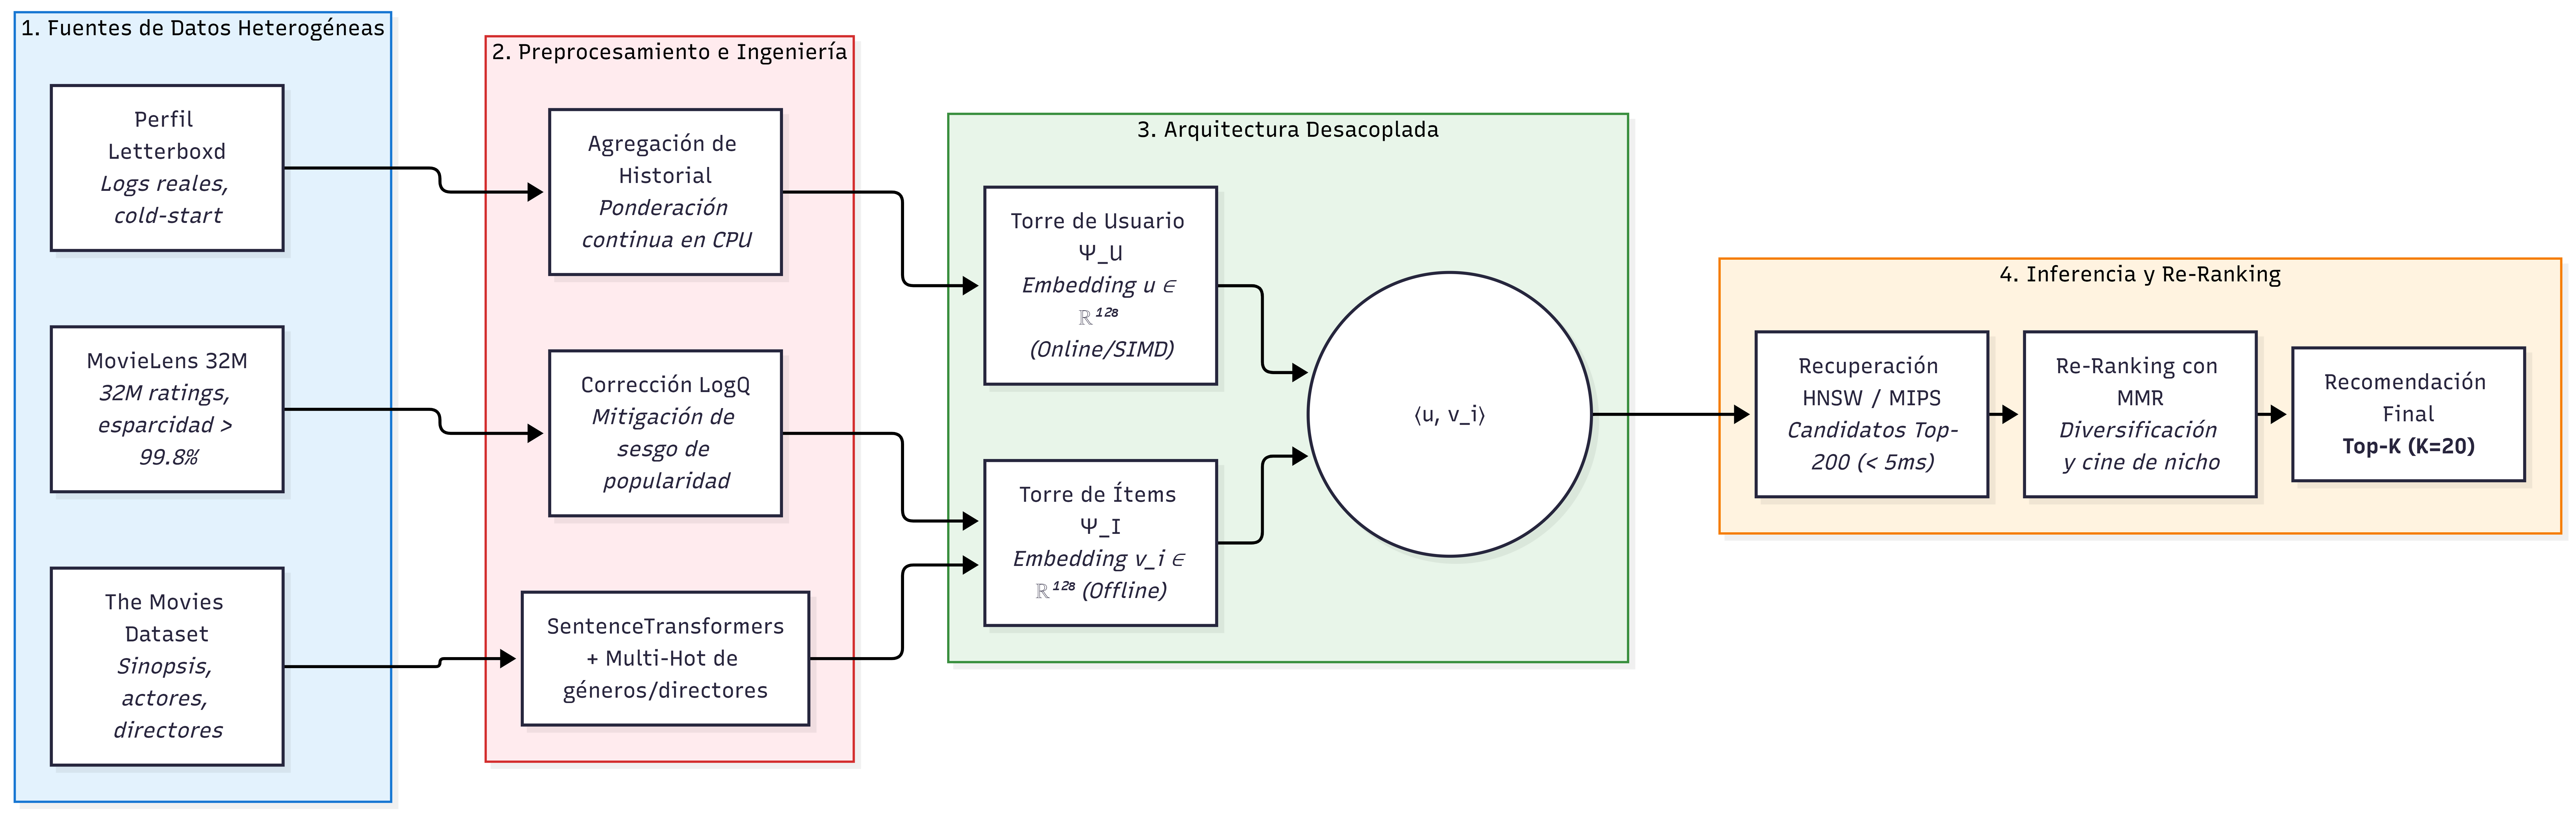
\includegraphics[width=0.82\textwidth]{diagrama_problema_M.png}
    \caption{Esquema conceptual del problema: integración de datos masivos y heterogéneos, modelado desacoplado y pipeline de inferencia eficiente en dos fases.}
    \label{fig:diagrama_problema}
\end{figure}
% ==========================================
% SECCIÓN 2: FUENTES DE DATOS
% ==========================================
\section{Identificación y Caracterización de las Fuentes de Datos}

Para abordar simultáneamente el modelado colaborativo, el arranque en frío y el sesgo de popularidad, el proyecto recurre a la combinación y cruce relacional de tres conjuntos de datos heterogéneos (Tabla \ref{tab:resumen_datasets}):

\begin{table}[!htbp]
    \centering
    \small
    \setlength{\tabcolsep}{5pt}
    \caption{Especificaciones cuantitativas de los conjuntos de datos analizados.}
    \label{tab:resumen_datasets}
    \begin{tabularx}{\textwidth}{p{4.3cm} c c X >{\centering\arraybackslash}p{2.5cm}}
        \toprule
        \textbf{Fuente de Datos} & \textbf{Usuarios ($N$)} & \textbf{Ítems ($M$)} & \textbf{Volumen / Registros} & \textbf{Dispersión} \\ 
        \midrule
        \textbf{MovieLens 32M} & $200\,948$ & $84\,432$ & $32\,000\,204$ ratings & $99.811\%$ \\
        \textbf{The Movies Dataset (TMDB)} & --- & $45\,466$ & Metadatos y sinopsis & --- \\
        \textbf{Letterboxd Export Format} & Perfil real & Catálogo & Secuencia temporal & Específico \\ 
        \bottomrule
    \end{tabularx}
\end{table}

\subsection{MovieLens 32M: Núcleo Cuantitativo Colaborativo}
Publicado por GroupLens Research en su versión oficial más exhaustiva \cite{movielens}, recoge el comportamiento continuado de usuarios hasta octubre de 2023. Proporciona:
\begin{itemize}
    \item \textbf{\texttt{ratings.csv}} ($\approx 700$ MB): Registros estructurados en cuádruplas $(\text{userId}, \text{movieId}, \text{rating}, \text{timestamp})$. Las calificaciones abarcan una escala ordinal de 10 niveles discretos (de 0.5 a 5.0 con incrementos de 0.5 estrellas).
    \item \textbf{\texttt{links.csv}}: Tabla relacional fundamental que asocia el identificador interno \texttt{movieId} con las claves de \texttt{imdbId} y \texttt{tmdbId}, actuando como puente de enlace hacia la información semántica.
\end{itemize}

\subsection{Análisis Empírico de la Distribución de Datos}
El procesamiento directo de los 32 millones de registros revela dos propiedades estadísticas críticas que condicionan el diseño del sistema (Figura \ref{fig:distribucion_ratings}):

\begin{enumerate}
    \item \textbf{Concentración extrema en la cola pesada (\textit{Long-Tail}):} Del catálogo evaluado ($84\,432$ películas con al menos un voto), el $10\%$ superior de títulos más populares ($8\,443$ filmes) concentra el \textbf{95.70\% de todas las interacciones del sistema}. El $90\%$ restante del inventario se reparte únicamente el $4.30\%$ de las calificaciones registradas. Cualquier modelo optimizado sin regularización de popularidad tenderá a ignorar este $90\%$ del inventario.
    \item \textbf{Asimetría de calificaciones (\textit{Positive Skew}):} Las notas otorgadas presentan una clara asimetría hacia valores positivos: las notas $\ge 3.5$ representan la gran mayoría del volumen total. Esto confirma que el usuario tiende a ver y calificar títulos que espera disfrutar, haciendo aconsejable tratar las notas altas como retroalimentación implícita de afinidad y ponderar el historial.
\end{enumerate}

\begin{figure}[!htbp]
    \centering
    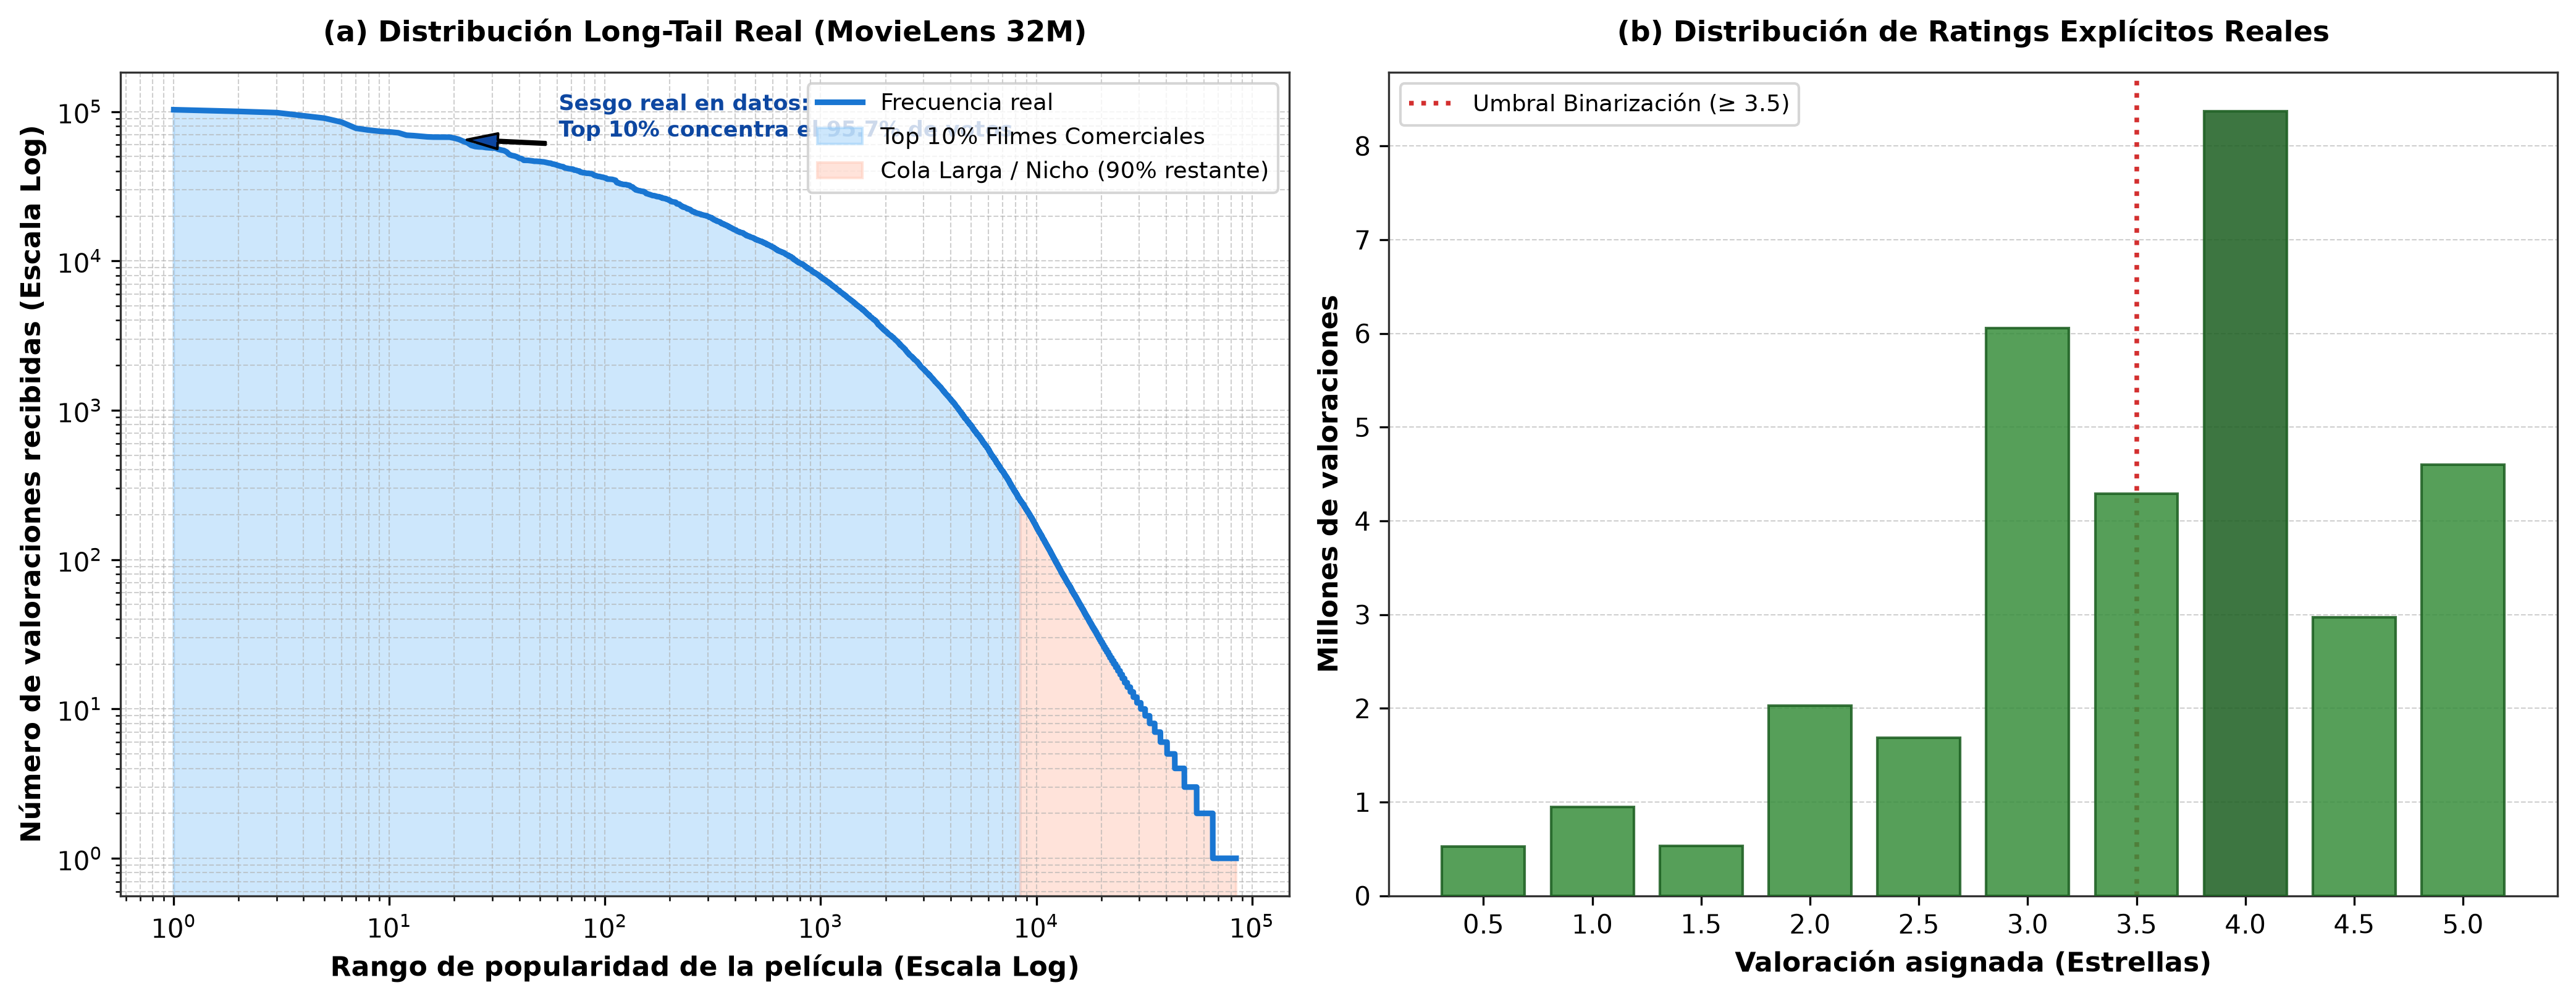
\includegraphics[width=0.78\textwidth]{distribucion_ratings.png}
    \caption{Distribución empírica obtenida sobre MovieLens 32M: (a) curva de potencia con el $95.70\%$ de interacciones concentradas en el Top 10\%, y (b) histograma de calificaciones con sesgo positivo.}
    \label{fig:distribucion_ratings}
\end{figure}

\subsection{The Movies Dataset (TMDB) y Metadatos Semánticos}
Para dotar de contexto intrínseco al sistema y solventar el arranque en frío, se integran los metadatos de The Movie Database:
\begin{itemize}
    \item \textbf{Atributos descriptivos y sinopsis (\texttt{movies\_metadata.csv}):} Texto narrativo (\textit{overview}), año de estreno, presupuestos y géneros cinematográficos.
    \item \textbf{Cuerpo técnico y reparto (\texttt{credits.csv}):} Directores, guionistas, equipo de fotografía y actores principales representados en estructuras tabulares deserializadas.
    \item \textbf{Palabras clave argumentales (\texttt{keywords.csv}):} Descriptores temáticos para enriquecer el perfil semántico.
\end{itemize}

\subsection{Letterboxd Export Format: Caso de Uso en Entorno Real}
Para validar el sistema en un entorno real de explotación, se adopta el esquema de exportación de Letterboxd (\texttt{watched.csv}, \texttt{ratings.csv}, \texttt{diary.csv}). Esto permite recrear el escenario en el que un usuario nuevo introduce su diario cinematográfico personal cronológico, permitiendo medir la latencia y la calidad de la recomendación ante perfiles no incluidos en el entrenamiento inicial.

\begin{table}[!htbp]
    \centering
    \small
    \setlength{\tabcolsep}{5pt}
    \caption{Esquema de integración y normalización relacional de atributos.}
    \label{tab:pipeline_datos}
    \begin{tabularx}{\textwidth}{p{2.5cm} p{2.8cm} X p{3.0cm}}
        \toprule
        \textbf{Dataset Origen} & \textbf{Campo Crudo} & \textbf{Transformación / Ingeniería de Atributos} & \textbf{Uso en el Modelo} \\ 
        \midrule
        MovieLens & \texttt{movieId}, \texttt{rating} & Binarización implícita ponderada por $r_{ui}$ & Torre de Usuario \\
        TMDB & \texttt{overview} & Embedding semántico denso ($d=384$) con MiniLM & Torre de Ítems \\
        TMDB & \texttt{genres}, \texttt{director} & Codificación dispersa Multi-Hot & Torre de Ítems \\
        MovieLens & \texttt{links.csv} & Mapeo relacional (\texttt{tmdbId} $\leftrightarrow$ \texttt{movieId}) & Fusión de datos \\
        Letterboxd & \texttt{diary.csv} & Secuencia cronológica y agregación online & Inferencia en tiempo real \\
        \bottomrule
    \end{tabularx}
\end{table}

% ==========================================
% SECCIÓN 3: ESTADO DEL ARTE
% ==========================================
\section{Estado del Arte y Soluciones Habituales}

Para entender cómo abordar el catálogo de MovieLens y TMDB sin incurrir en cuellos de botella de memoria o latencia, revisamos las soluciones más representativas utilizadas en la literatura y en la industria:

\subsection{¿Qué se hace habitualmente? Enfoques y Casos Reales}
\begin{enumerate}
    \item \textbf{Factorización Matricial (SVD / ALS) --- Caso Netflix Prize:}
    Popularizado por Koren et al. \cite{koren2009} durante la célebre competición del \textit{Netflix Prize}. Funciona bien descomponiendo la matriz de valoraciones numéricas en factores latentes, pero es un modelo estrictamente colaborativo: ignora por completo el texto de las sinopsis de TMDB y no puede recomendar nada a un usuario nuevo sin historial previo (\textit{cold-start}).

    \item \textbf{Autoencoders Lineales (EASE$^R$) --- Caso Harald Steck (Netflix):}
    Propuesto por Harald Steck \cite{steck2019} en Netflix y muy utilizado como solución de referencia en competiciones de Kaggle por su precisión inmediata. Su gran inconveniente con nuestro catálogo es de memoria: exige calcular e invertir una matriz de tamaño catálogo $\times$ catálogo ($M \times M$). Con más de $84\,000$ películas, almacenar dicha matriz requiere más de 28~GB de memoria RAM, haciendo inviable su ejecución en un ordenador convencional.

    \item \textbf{Redes Neuronales Acopladas (NeuMF / NCF):}
    Introducido por He et al. \cite{he2017}, combina vectores latentes con capas densas no lineales. Aunque es un referente académico, en producción presenta un cuello de botella crítico: para recomendar películas debe pasar al usuario y al ítem juntos por toda la red. Evaluar esa red neuronal $84\,000$ veces por cada usuario en tiempo real destruye cualquier posibilidad de respuesta interactiva rápida.

    \item \textbf{Modelos sobre Grafos (LightGCN):}
    Propuesto por He et al. \cite{he2020}, modela usuarios y películas como nodos interconectados de un grafo bipartito. Si bien captura muy bien la estructura comunitaria, mantener millones de aristas dispersas en memoria dificulta una paralelización limpia y vectorizada en CPU bajo recursos limitados.

    \item \textbf{Arquitectura de Dos Torres (\textit{Two-Tower}) --- Caso YouTube / Google:}
    Diseñada por Covington et al. \cite{covington2016} y formalizada por Yi et al. \cite{yi2019} para el motor de recomendaciones a gran escala de YouTube. Separa el sistema en dos ramas independientes: una procesa al usuario y otra los metadatos de las películas. Esto permite precomputar los vectores de todo el catálogo una sola vez y resolver la búsqueda en milisegundos mediante índices vectoriales rápidos en memoria RAM (como FAISS de Meta).

    \item \textbf{Diversificación con MMR --- Caso Motores de Búsqueda y Noticias:}
    Formulado originalmente por Carbonell y Goldstein \cite{carbonell1998}, es el estándar para evitar que la lista final sea monótona o redundante (por ejemplo, recomendar cinco secuelas de la misma saga), reequilibrando afinidad con variedad temática y cine de nicho.
\end{enumerate}

\begin{table}[!htbp]
    \centering
    \small
    \setlength{\tabcolsep}{5pt}
    \caption{Comparativa práctica de paradigmas frente a las restricciones del proyecto.}
    \label{tab:comparativa_modelos}
    \begin{tabularx}{\textwidth}{p{2.6cm} p{3.2cm} c X c}
        \toprule
        \textbf{Enfoque} & \textbf{Referencia / Caso Real} & \textbf{Cold-Start} & \textbf{Metadatos (TMDB)} & \textbf{Viabilidad en CPU} \\ 
        \midrule
        \textbf{SVD / ALS} & Netflix Prize \cite{koren2009} & Nulo & No compatible (solo notas) & Alta (lineal) \\
        \textbf{EASE$^R$} & Harald Steck (Netflix) \cite{steck2019} & Nulo & No compatible & Inviable ($>28$ GB RAM) \\
        \textbf{NeuMF} & He et al. \cite{he2017} & Bajo & Posible pero costoso & Muy lenta en tiempo real \\
        \textbf{LightGCN} & He et al. \cite{he2020} & Bajo & Requiere grafos complejos & Media (acceso disperso) \\
        \textbf{Two-Tower} & YouTube / Google \cite{yi2019} & \textbf{Excelente} & \textbf{Nativo (texto y géneros)} & \textbf{Óptima (SIMD / FAISS)} \\ 
        \bottomrule
    \end{tabularx}
\end{table}

% ==========================================
% SECCIÓN 4: JUSTIFICACIÓN TECNOLÓGICA
% ==========================================
\section{Justificación Tecnológica del Enfoque Propuesto}

Para responder a las limitaciones observadas en los datos (dispersión del $99.8\%$, arranque en frío y concentración del $95.70\%$ en superventas) garantizando respuesta en milisegundos en CPU, se propone un flujo en **dos etapas desacopladas** (Figura \ref{fig:arquitectura_two_tower}):

\begin{figure}[!htbp]
    \centering
    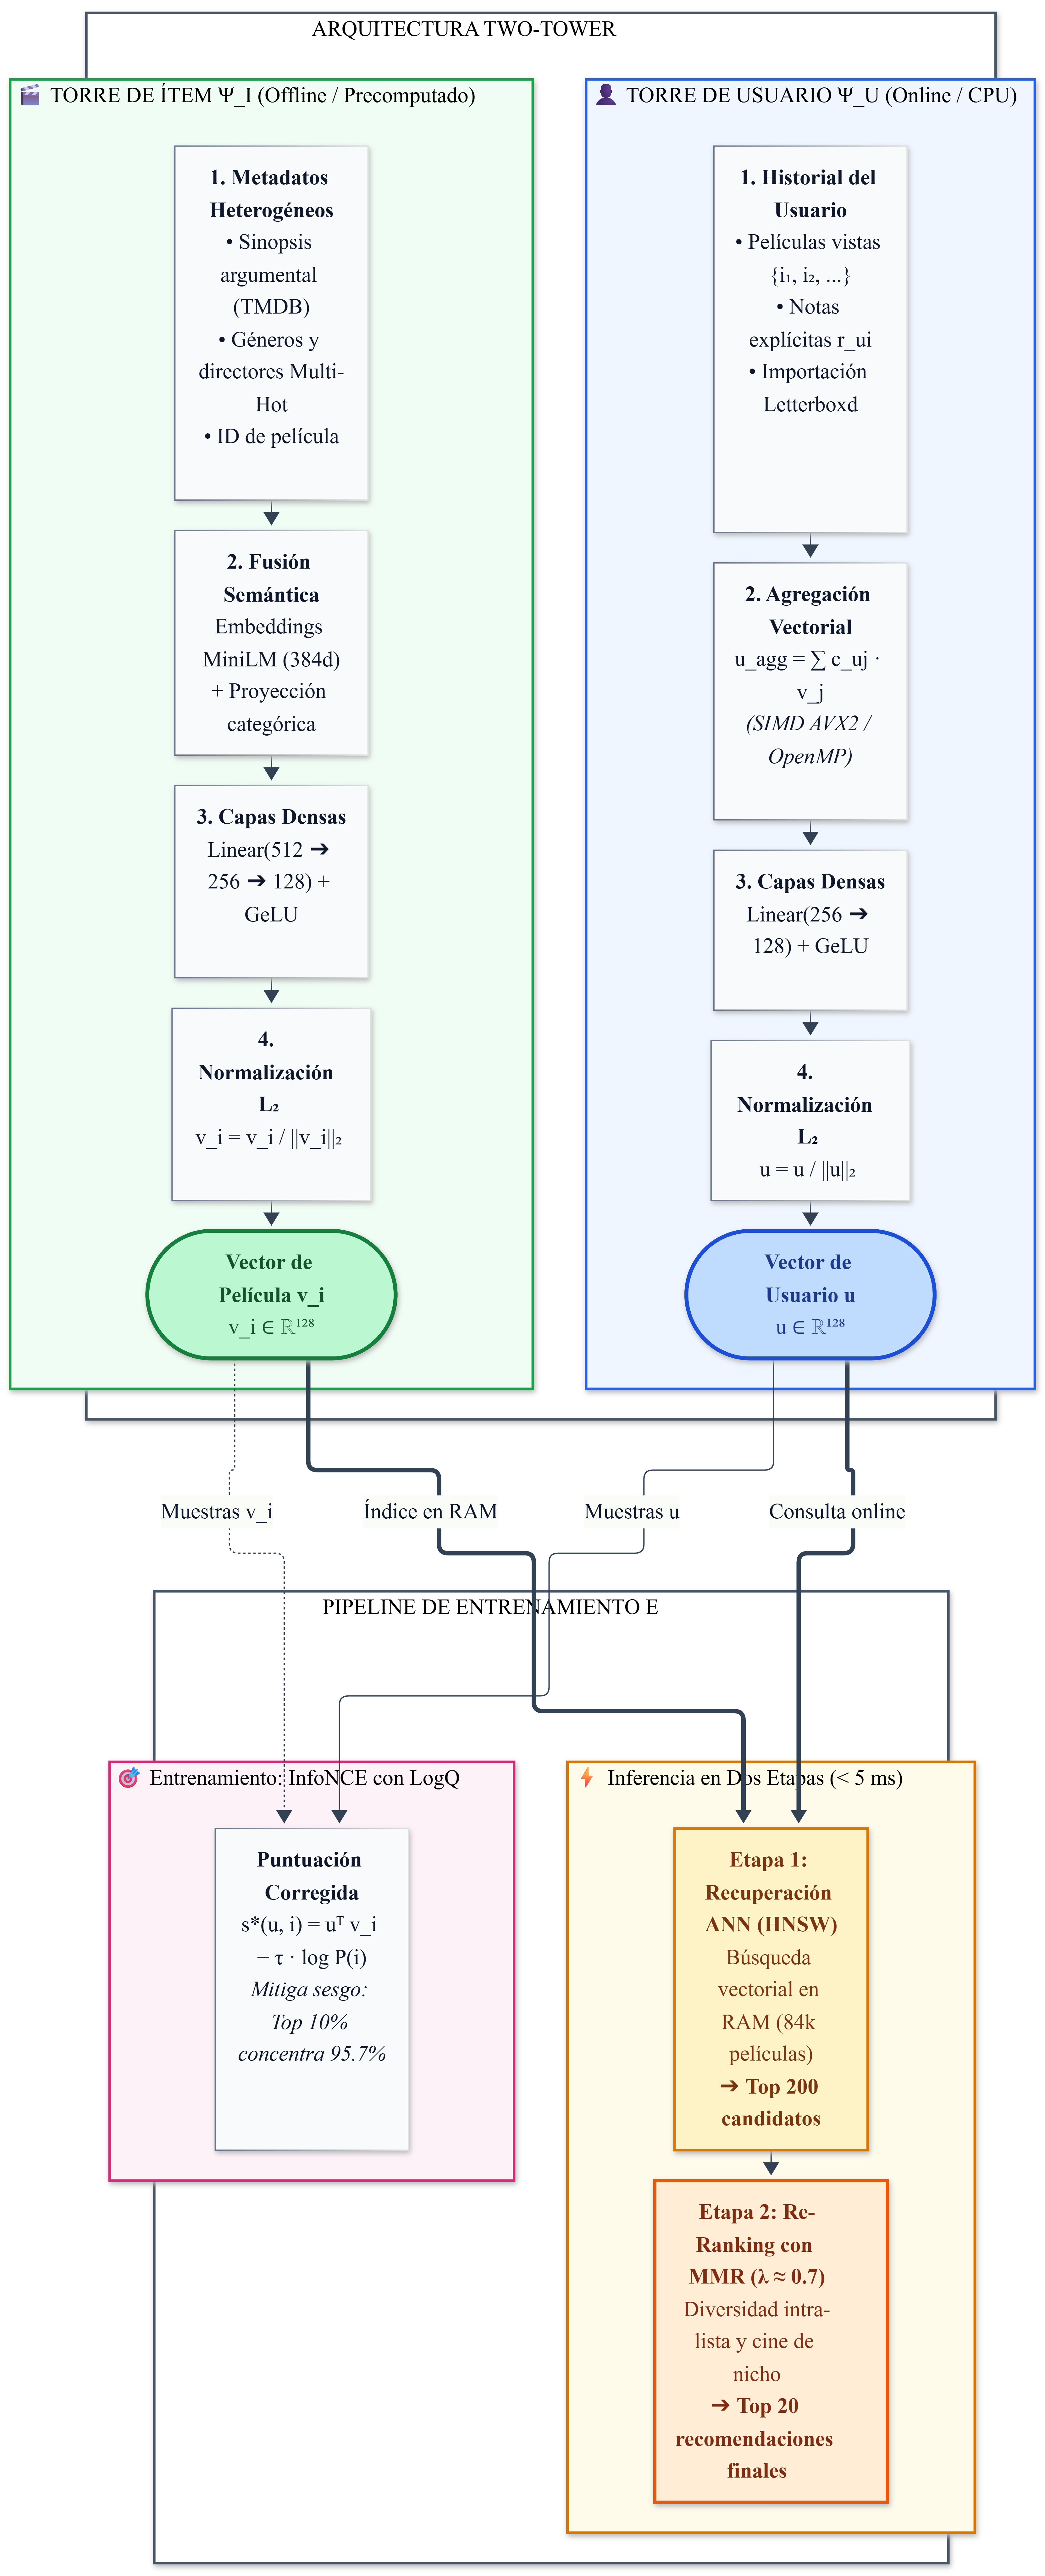
\includegraphics[width=0.60\textwidth]{arquitectura_two_tower_Mv.png}
    \caption{Arquitectura propuesta: desacoplamiento en dos etapas (Recuperación Two-Tower con búsqueda vectorial ANN y Reordenamiento con diversificación MMR).}
    \label{fig:arquitectura_two_tower}
\end{figure}

\subsection{Etapa 1: Recuperación Rápida con Red de Dos Torres (\textit{Two-Tower})}
El modelo separa la representación del usuario y de las películas en dos redes independientes que proyectan a un espacio común de dimensión $d = 128$:
\begin{equation}
    \hat{s}(u, i) = \langle \mathbf{u}, \mathbf{v}_i \rangle = \Psi_U(\mathbf{x}_u)^\top \Psi_I(\mathbf{x}_i)
    \label{eq:two_tower}
\end{equation}

Esta separación resuelve tres problemas clave del catálogo:
\begin{enumerate}
    \item \textbf{Arranque en frío resuelto por metadatos:} La Torre de Ítem ($\Psi_I$) genera el vector $\mathbf{v}_i$ combinando sinopsis textuales (vía \textit{SentenceTransformers}) con directores y géneros de TMDB. Una película recién estrenada sin votos obtiene una representación válida de inmediato.
    \item \textbf{Inferencia en milisegundos sobre 84\,000 películas:} Los vectores $\mathbf{v}_i$ de todo el catálogo se precomputan offline y se indexan en RAM (apenas 43~MB). En tiempo real solo se evalúa la Torre de Usuario ($\Psi_U$) para obtener $\mathbf{u}$ y extraer los $K_c = 200$ títulos más afines en menos de 5~ms mediante búsqueda vectorial aproximada (\textit{HNSW}).
    \item \textbf{Mitigación del sesgo de popularidad (LogQ):} Durante el entrenamiento contrastivo, se resta la probabilidad marginal de aparición del filme ($s^* = \mathbf{u}^\top \mathbf{v}_i - \tau \log P(i)$) según Yi et al. \cite{yi2019}. Esto evita que los títulos comerciales acaparen artificialmente las recomendaciones.
\end{enumerate}

\subsection{Etapa 2: Diversificación y Descubrimiento con MMR}
La primera etapa prioriza relevancia pura, lo que suele devolver películas muy similares entre sí (por ejemplo, varias entregas de la misma saga). Para introducir variedad y rescatar cine de calidad de la cola larga, se aplica Relevancia Marginal Máxima \cite{carbonell1998} sobre los 200 candidatos:
\begin{equation}
    i^* = \arg\max_{i \in \mathcal{C} \setminus \mathcal{S}} \left[ \lambda \cdot \text{Score}(u, i) - (1 - \lambda) \max_{j \in \mathcal{S}} \text{Sim}(\mathbf{v}_i, \mathbf{v}_j) \right]
    \label{eq:mmr}
\end{equation}
Fijando $\lambda \approx 0.7$, el algoritmo equilibra afinidad personal y novedad temática, produciendo la lista final de $K = 20$ recomendaciones.

% ==========================================
% SECCIÓN 5: PLAN DE COMPUTACIÓN PARALELA
% ==========================================
\section{Plan de Computación Paralela y Optimización HPC (CPIA)}

El diseño traslada el cómputo crítico a operaciones vectoriales continuas en CPU, ideales para explotación multihilo y vectorización:

\begin{enumerate}
    \item \textbf{Paralelización multihilo con OpenMP en C/C++:} El cálculo concurrente de perfiles de usuario y la evaluación masiva de similitudes se distribuirá entre núcleos con balanceo dinámico \cite{openmp}:
\begin{lstlisting}
#pragma omp parallel for schedule(dynamic, 64)
for (int u = 0; u < num_usuarios; ++u) {
    calcular_perfil_usuario(&usuarios[u], items_db, dim_embedding);
    evaluar_similitudes_simd(&usuarios[u], candidatos, top_k);
}
\end{lstlisting}
    \item \textbf{Vectorización SIMD (AVX2 / AVX-512):} Dado que los embeddings tienen tamaño fijo ($d = 128$), los productos escalares $\langle \mathbf{u}, \mathbf{v}_i \rangle$ se optimizarán en memoria alineada usando instrucciones intrínsecas FMA (8 a 16 operaciones float por ciclo por núcleo).
    \item \textbf{Evaluación de escalabilidad:} En las siguientes entregas se medirá el \textit{Speedup} experimental $S_p = T_1 / T_p$ y la eficiencia para $p \in \{1, 2, 4, 8, 16\}$ hilos frente a la cota teórica de la Ley de Amdahl.
\end{enumerate}

% ==========================================
% SECCIÓN 6: CONCLUSIONES
% ==========================================
\section{Conclusiones y Próximos Pasos}

Esta propuesta establece la viabilidad técnica del motor de recomendación tras caracterizar empíricamente los retos de MovieLens 32M (dispersión del $99.81\%$ y el $95.70\%$ de interacciones concentradas en solo el $10\%$ del catálogo). La integración con los metadatos de TMDB y el formato de Letterboxd proporciona el contexto necesario para superar el arranque en frío en un entorno real.

La arquitectura Two-Tower complementada con reordenamiento MMR ofrece el equilibrio óptimo para el proyecto: desacopla el cálculo pesado, acota el uso de memoria RAM a decenas de megabytes y traslada las operaciones críticas a rutinas de álgebra vectorial idóneas para su implementación paralela en C++ con OpenMP y SIMD. En la próxima entrega (E2) se abordará el pipeline de preprocesamiento, la generación de embeddings y el desarrollo de los benchmarks de rendimiento en CPU.

% ==========================================
% BIBLIOGRAFÍA
% ==========================================
\begin{thebibliography}{99}
\small
\setlength{\itemsep}{2pt}
\setlength{\parskip}{0pt}

\bibitem{movielens}
Harper, F. M., \& Konstan, J. A. (2015). \textit{The MovieLens Datasets: History and Context}. ACM Transactions on Interactive Intelligent Systems (TiiS), 5(4), 1--19.

\bibitem{koren2009}
Koren, Y., Bell, R., \& Volinsky, C. (2009). \textit{Matrix Factorization Techniques for Recommender Systems}. IEEE Computer, 42(8), 30--37.

\bibitem{covington2016}
Covington, P., Adams, J., \& Sargin, E. (2016). \textit{Deep Neural Networks for YouTube Recommendations}. Proceedings of the 10th ACM Conference on Recommender Systems (RecSys '16), 191--198.

\bibitem{he2017}
He, X., Liao, L., Zhang, H., Nie, L., Hu, X., \& Chua, T. S. (2017). \textit{Neural Collaborative Filtering}. Proceedings of the 26th International Conference on World Wide Web (WWW '17), 173--182.

\bibitem{liang2018}
Liang, D., Krishnan, R. G., Hoffman, M. D., \& Jebara, T. (2018). \textit{Variational Autoencoders for Collaborative Filtering}. Proceedings of the 2018 World Wide Web Conference (WWW '18), 687--696.

\bibitem{kang2018}
Kang, W. C., \& McAuley, J. (2018). \textit{Self-Attentive Sequential Recommendation}. IEEE International Conference on Data Mining (ICDM '18), 197--206.

\bibitem{steck2019}
Steck, H. (2019). \textit{Embarrassingly Shallow Autoencoders for Sparse Data}. Proceedings of the World Wide Web Conference (WWW '19), 3251--3257.

\bibitem{yi2019}
Yi, X., Yang, J., Hong, L., Cheng, D. Z., Heldt, L., Kumthekar, A., Zhao, Z., Wei, L., \& Chi, E. (2019). \textit{Sampling-Bias-Corrected Neural Modeling for Large Corpus Item Recommendations}. Proceedings of the 13th ACM Conference on Recommender Systems (RecSys '19), 269--277.

\bibitem{he2020}
He, X., Deng, K., Wang, X., Li, Y., Zhang, Y., \& Wang, M. (2020). \textit{LightGCN: Simplifying and Powering Graph Convolution Network for Recommendation}. Proceedings of the 43rd International ACM SIGIR Conference, 639--648.

\bibitem{carbonell1998}
Carbonell, J., \& Goldstein, J. (1998). \textit{The Use of MMR, Diversity-Based Reranking for Reordering Documents and Producing Summaries}. Proceedings of the 21st Annual International ACM SIGIR Conference, 335--336.

\bibitem{openmp}
OpenMP Architecture Review Board. (2018). \textit{OpenMP Application Programming Interface Version 5.0}. Technical Report.

\end{thebibliography}

\end{document}